%%
%% @filename rapport.tex
%% @date 2023-11-22 14:10
%% @author Nemo D'ACREMONT and Martin EYBEN <nemo.d'acremont@enseirb-matmeca.fr> and <martin.eyben@enseirb-matmeca.fr>
%% @brief ...
%%
\documentclass{customClass}

%----------- Informations du rapport ---------
\title{Rapport Projet 1 -- Munificence}
\author{Nemo D'ACREMONT, Martin EYBEN}

\titre{Rapport Projet 1 -- Munificence} % Titre du fichier

\lieuprojet{Enseirb-Matmeca -- I1} % Pour le bas de la page
\basdepage{Munificence}
\eleve{Nemo D'ACREMONT, Martin EYBEN}
\sujetprojet{Munificence}

\dates{
    S5 - Année universitaire 2023-2024
}
\shortdates{2023-2024}

\graphicspath{{./img}}


\begin{document}

%
%  Page de garde
%
\mainPage
\tableofcontents{}
\pagebreak{}

% Initialisation 

\fairemarges

%
%  Parties
%
\setcounter{section}{0}  % Fait joli


%
%  Introduction
%


\section*{Préambule}
\addcontentsline{toc}{section}{Préambule}

% Ceci est une introduction, jsp quoi dire, Martin est nul

% Cependant, je ne pense pas que l'on devrait faire une partie par élément du projet, je ne suis pas sûr que ce soit ce que le rapport doit être
% En fait, je ne pense pas qu'on doive être exhaustif, évoquer les parties intéressantes devrait être suffisant


Ce projet avait pour objectif la mise en oeuvre de notions étudiées tout au long du premier 
semestre, à la création d'un jeu plus ou moins inspiré du jeu de société "Splendor". 

Il s'agissait dans un premier temps de mettre en place les fondamentaux du jeu, puis de les 
étendre plus ou moins artificiellement, nous forçant à faire preuve de rigueur dans nos
méthodes et à mobiliser nos connaissances algorithmiques de façon à aborder sereinement les
problèmes que nous rencontrions.







\section{Organisation du projet}


% Travail en équipe
\subsection{Organisation du travail en équipe}

% Problématique
\subsubsection*{Problématique}

    Le travail en équipe n'est pas une chose évidente, et il est nécessaire de mettre en
place une méthode afin d'optimiser notre productivité, sinon cas nous le risque de 
malencontreusement traiter d'un même sujet séparément, et se rendre compte qu'on a perdu notre
temps.

% Solutions
\subsubsection*{Solutions mises en place}

\subsubsection*{Méthode Kanban}

    Nous avons utilisé l'application web kanboard, installée sur un serveur personnel, afin de
distribuer le travail à faire, ainsi nous savions à tout moment, ce qu'il y avait à faire,
ce qui était en train d'être fait et ce qui avait été fait. 


\subsubsection*{Utilisation de git}

    L'utilisation d'un gestionnaire de version est essentiel pour la 
réalisation de ce genre de projet. Cependant, se limiter à une utilisation élémentaire
de ce logiciel pour le travail en équipe peut mener à une multiplication de problèmes de 
conflits, pouvant entraver l'avancée du projet. 

    Plusieurs solutions plus ou moins élaborées pouvaient être mises en place, nous avons opté 
pour un entre-deux: nous utilisions 3 branches : la branche master, qui se devait d'être 
propre, le code qui s'y trouvait devait toujours être
compilable, et devait contenir le moins de bugs possible. Les deux autre branches que nous
utilisions nous étaient attitrées, à chaque fois que nous nous attribuions une tache sur le
kanboard, nous développions une solution sur notre branche puis nous fusionnions sur la branche
master.

Schématiquement, notre utilisation de git se résume au schéma suivant :

\begin{center}
    \begin{figure}[H]
        \centering
        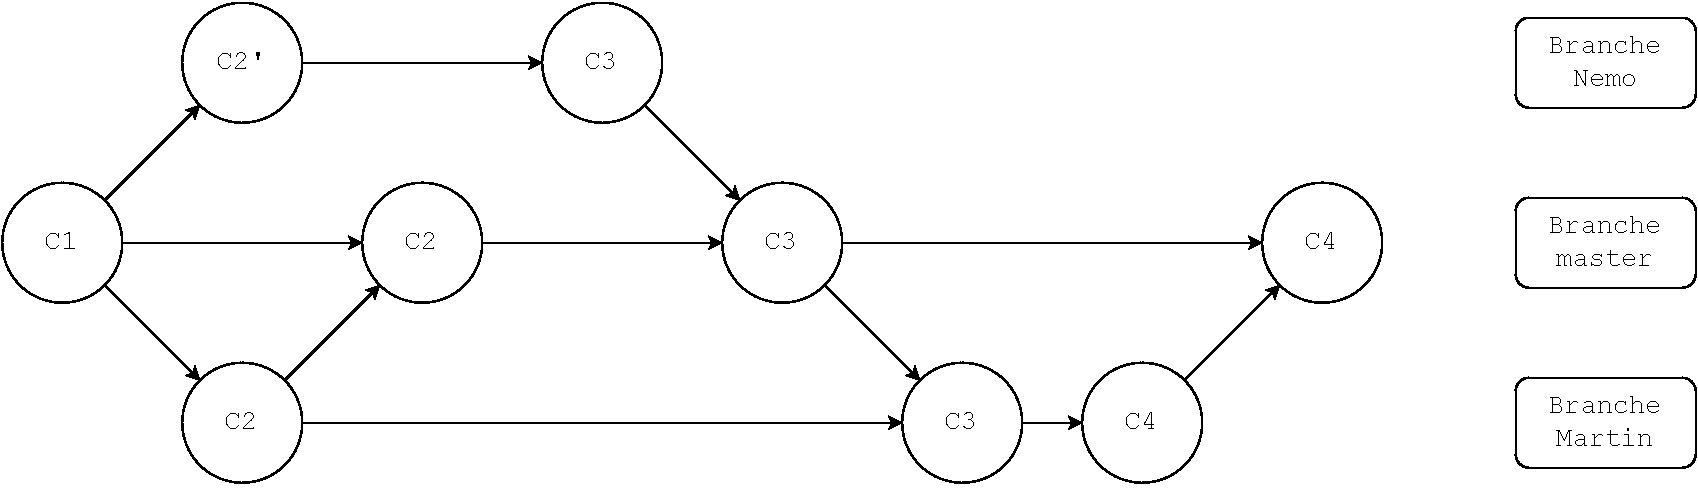
\includegraphics[width=\textwidth]{img/git_branch.pdf}
        \caption{Utilisation de nos 3 branches de git}
        \label{fig:git_branch}
    \end{figure}
\end{center}


% Organisation Code
\subsection{Organisation du code}


\subsubsection*{Problématique}


    Un projet d'une telle envergure nécessite une organisation spéciale afin d'être mené à 
bien. Il s'agit d'une organisation qui doit faciliter l'ajout de nouvelle fonctionnalités,
faciliter la modification de fonctionnalités déjà présente et faciliter la lecture et la 
compréhension de ce qui a déjà été fait.




\subsubsection*{Solutions mises en place}


\subsubsection*{Division en dossiers principaux}


    Sachant que nous nous apprêtions à créer un exécutable pour le projet en lui-même et pour les
tests, nous avons décidé de séparer les sources pour chaque exécutable dans un dossier séparé.


    Ainsi, notre projet est constitué de 4 dossiers principaux: \code{/src}, \code{/tst}, 
\code{/cli\_src}, \code{/evaluator\_src}, comme le schématise le schéma ci-dessous


\begin{center}
    \begin{figure}[H]
        \centering
        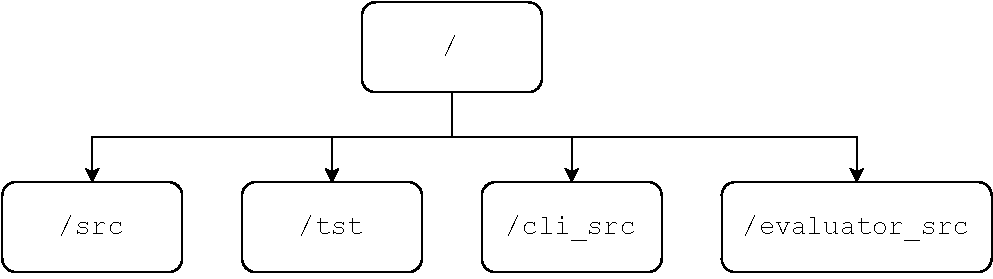
\includegraphics[width=.5\textwidth]{img/main_directories.pdf}
        \caption{Schéma des dossiers principaux du projet}
        \label{fig:main_dirs}
    \end{figure}
\end{center}




\subsubsection*{Division du code par thème}


    Une fois qu'on a divisé en dossiers principaux, on divise le code
dans des sous-dossiers au sein de ces dossiers. Ainsi, on va avoir un
sous-dossier pour les builders et la structure de guilde, un pour les 
tokens et la structure de markets etc... On a aussi un sous-dossier \code{/src/utils},
qui va contenir toutes les structures et fonctions génériques, comme
une structure de file ou une macro \code{MIN} qui retourne le minimum entre 2 entiers.

    L'architecture des sous-dossiers de \code{/src} est schématisé ci-dessous :


\begin{center}
    \begin{figure}[H]
        \centering
        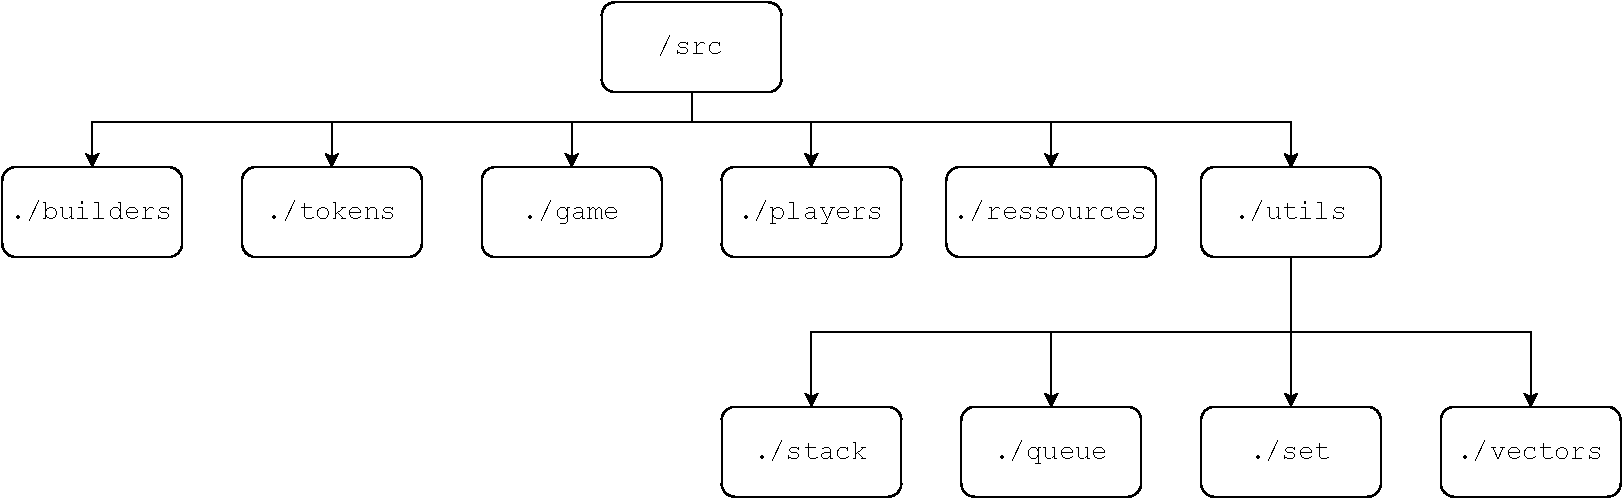
\includegraphics[width=.8\textwidth]{img/src_sub_dir.pdf}
        \caption{Schéma sous-dossiers de $/src$}
        \label{fig:src_sub_dirs}
    \end{figure}
\end{center}




\subsubsection*{Mise en place d'une convention}


\subsubsection*{Problématique}


    Le travail en groupe fait qu'on se retrouve tôt ou tard à lire ou à utiliser des outils codés par une 
autre personne. Ainsi, la forme du code requiert une certaine attention afin de rendre l'utilisation de ces
outils naturelle et la lecture du code uniforme.


\subsubsection*{Solution mis en place}

    Pour résoudre ce problème de forme, on a mit en place une convention de nommage pour les
variables et les fonctions, ainsi que des règles d'écriture. 

    Nous avons décidé d'utiliser la convention \code{snake\_case} pour ce qui est de la forme,
nous nommons les types \lstinline{struct type_t} afin de ne pas les confondre avec d'éventuelles variables.
Une fonction qui devait s'appliquer à un type \lstinline{struct type_t} en particulier est notée
\lstinline{type_function(...)}.

    Vous trouverez ci-dessous des exemples non-exhaustif de la mise en pratique de ces conventions

\begin{lstlisting}[frame=single, caption={Exemples de mise en pratique de ces conventions}]
struct queue_t ;


unsigned int queue_append(struct queue_t* queue, void* value);
\end{lstlisting}




\subsubsection*{Compilation}


\subsubsection*{Problématique}


    Travailler avec telle structure de fichier rend la compilation moins évidente, et fastidieuse si on voulait 
la faire manuellement avec \code{gcc}.


\subsubsection*{Solution mis en place}

    Nous avons utilisé \code{make}, et nous nous sommes appliqué à l'écriture d'un \code{makefile} qui
permettrait d'avancer sereinement dans le projet.

    Notons avant tout que notre \code{makefile} est largement inspiré des ébauches proposées du \href{https://spin.atomicobject.com/makefile-c-projects/}{poste de blog de Job Vranish}, 
ces ébauches formait une fondation solide sur laquelle travailler. Cependant, nous nous sommes tout de même donné le mal de nous l'approprier
afin de l'adapter à notre structure peut-être originale.

    Comme la plupart des sources du dossier \code{/src} sont partagées entre chaque exécutables, nous avons fait le choix de
d'abord chercher tous les fichiers sources de \code{/src}, puis de retirer le fichier \code{/src/projet.c} contenant la fonction main.

\begin{lstlisting}[frame=single, language=sh, caption={Filtrage des fichiers sources du jeu}]
SRC_DIRS := ./src
PROJECT_MAIN_FILE_NAME := ./src/project.c

SRCS := $(shell find $(SRC_DIRS) -name '*.c')
SRCS := $(filter-out $(PROJECT_MAIN_FILE_NAME), $(SRCS))
\end{lstlisting}

    Nous avons opté pour l'utilisation de l'option \code{-Isous\_dossier} de \code{gcc}, permettant de déclarer des librairies systèmes. Ainsi, en 
l'utilisant avec tous les sous-dossiers de \code{/src} et des autres dossiers principaux, cela nous permet de nous limiter à l'écriture de `\lstinline[language=C]{#include "fichier.h"}` dans nos fichiers sources plutôt que le chemin relatif vers le fichier \code{fichier.h}. Étant donné notre arborescence complexe, cela simplifie largement la lecture et l'écriture des dépendances.

    Cependant, il fallait aussi que nos éditeurs, par le biais de clang, puissent être utilisable. D'où l'ajout de la target \code{clang\_custom\_lib\_support} dans
le makefile, permettant de créer le fichier de configuration \code{compile\_flags.txt} indiquant nos librairies systèmes personnalisées à clang.

Finalement l'utilisation d'un nouveau dossier, le dossier \code{/build}. Ce dernier nous sert à stocker tous les fichiers de compilation. Afin de les stocker, nous recréons la structure précédente du fichier, comme le schématise la figure \ref{fig:build_dir}. 

    L'utilisation de ce dossier permet d'avoir une séparation claire entre le reste du projet et la partie compilation.

\begin{center}
    \begin{figure}[H]
        \centering
        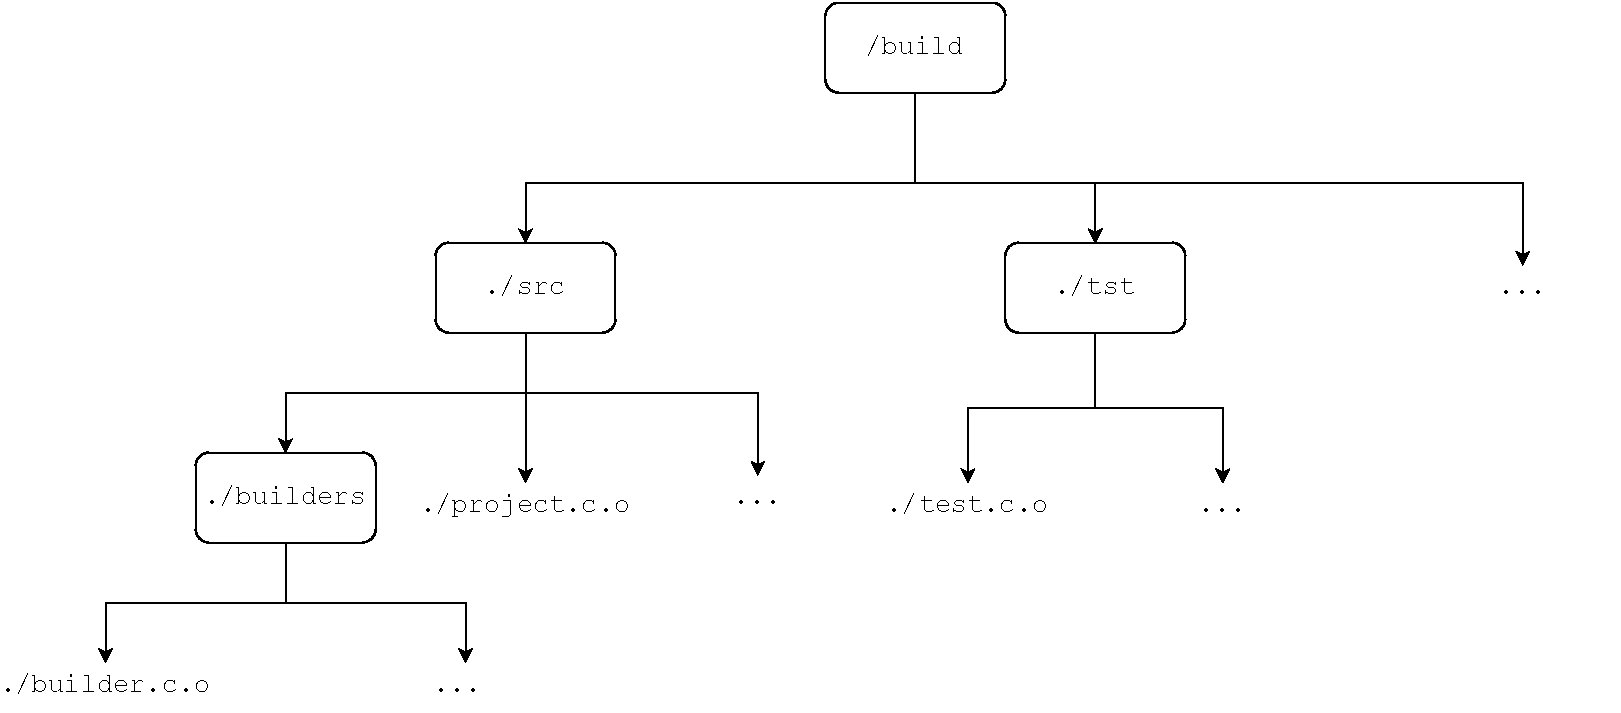
\includegraphics[width=.8\textwidth]{img/build_dir.pdf}
        \caption{Schéma arboressence du dossier /build}
        \label{fig:build_dir}
    \end{figure}
\end{center}




\subsection*{Structure d'une partie}

% Label pour le référencement
\label{game}

\subsection*{Problématique}

Le nerf du projet se trouve dans l'implémentation d'une partie. Elle doit permettre de jouer chaque tour séparément, connaître l'état du tour précédent et ainsi pouvoir avoir un historique de la partie. Ce qui sera notamment très utile lors de la création de l'interface mais aussi pour pouvoir jouer de manière indépendante plusieurs parties. (cf \ref{evaluator} et \ref{cli})
\subsection*{Architecture}

\subsubsection*{Structure de tour}

\begin{lstlisting}[frame=single, caption={Implémentation de la structure turn\_t}]
struct turn_t
{
	struct market_t market;
	struct guild_t guild;
	struct player_t players[MAX_PLAYERS];
	unsigned int current_player;
	unsigned int points_to_win;
	unsigned int display; /* Used to display in other functions*/
	unsigned int num_player;
	unsigned int id;
	struct game_parameters params;
	struct context context;
};
\end{lstlisting}

Chaque tour possède la copie de la partie à un instant t.\\
On y retrouve l'état du marché, de la guilde et les inventaires des joueurs à l'issue du tour. Mais également le contexte de ce qu'il s'est passé dans le tour (cf \ref{cli}).

Chaque tour possède volontairement beaucoup d'informations sur la partie car cela va permettre de jouer énormément avec ces paramètres lorsque l'utilise en paramètre de fonction (pour les faveurs et les pouvoirs notamment, cf \ref{skills}).

\subsubsection*{Structure de partie}

\begin{lstlisting}[frame=single, caption={Implémentation de la structure game\_t}]
struct game_t
{
    // +1 for the init state, +1 for the final state
    struct turn_t turns[MAX_MAX_TURNS + 1 + 1]; 
    unsigned int num_turns;
    unsigned int current_turn_index;
};
\end{lstlisting}

Chaque partie stocke l'ensemble des tours qui ont été joués, et contient au plus\\ MAX\_MAX\_TURNS tours (toujours pour éviter l'utilisation de \code{malloc} cf \ref{nomalloc}).\\
num\_turns indique le nombre de tours maximum de la partie (par défaut 10 mais peut être spécifié avec le paramètre -m) et current\_turn\_index l'indice du tour actuellement joué.

\subsection*{Fonctionnement d'une partie}

\subsubsection*{Initialisation de la partie}
Pour initialiser une nouvelle partie, on utilise la fonction \code{init\_game} avec les paramètres souhaités.
\lstset{language=C, style=code}
\begin{lstlisting}[frame=single]
/*
	Init game with params
*/
void init_game(struct game_t*, struct game_parameters);
\end{lstlisting}

\begin{lstlisting}[frame=single, caption={Structure des paramètres de la partie}]
struct game_parameters
{
	unsigned int max_turns;
	unsigned int points_to_win;
	unsigned int builder_seed;
	unsigned int market_seed;
	unsigned int random_seed;
	unsigned int display;
	unsigned int num_player;
};
\end{lstlisting}

La fonction \code{init\_game} modifie le premier tour de la partie en initialisant toutes les instances et en imposant les paramètres de la partie.\\
Le tour est alors sauvegardé (cf \ref{save}) et on peut lancer la partie avec \code{play\_game}.

\subsubsection*{Particularité de \code{rand}}
La fonction \code{rand} étant non ré-entrante, il s'agit de l'unique endroit où \code{srand} est appelée. \code{srand} est appelée une fois lors de l'initialisation des architectes (cf \ref{builders}) et une fois lors de l'initialisation des jetons (cf \ref{tokens}) afin de permettre la création de decks aléatoires indépendants. \\
\code{srand} est alors appelée une dernière fois avec \code{random\_seed} pour initialiser le hasard du reste des actions prises dans la partie.

\begin{figure}[H]
    \centering
    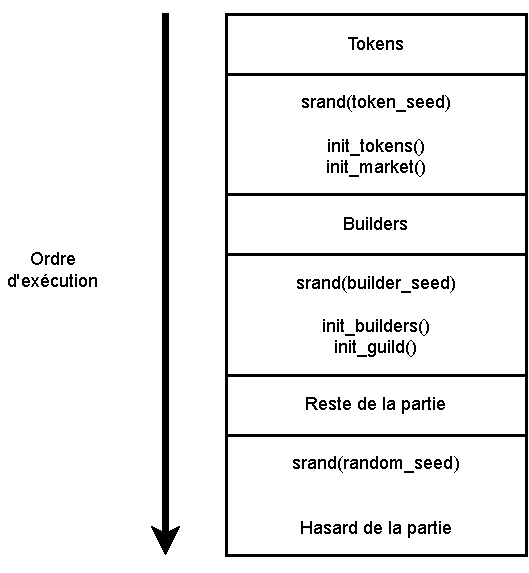
\includegraphics{img/utilisation_srand.pdf}
    \caption{Utilisation de \code{srand}}
    \label{fig:sranduse}
\end{figure}

\subsubsection*{Exécution d'un tour}

\begin{lstlisting}[frame=single, caption={Implémentation de l'exécution d'un tour}]
struct turn_statistics turn_play(struct turn_t* current_turn)
{
    /* Favors execution */
    
	/*
        Take a random decision and check if it's possible to hire a builder
	*/
	unsigned int random_choice = rand() % 100; 
	struct builder_t* builder_to_buy = select_affordable_builder(guild, current_player);

	if ((random_choice < 50) && (builder_to_buy != NULL)) 
	{
		  /* Hire builder and execute associated skills */ 
	}
	else if (random_choice < 90)
	{
		/* Pick tokens and execute associated skills  */
	}
	else 
	{
		/* Skip turn */
	}

}
\end{lstlisting}

A l'aide de la fonction \code{turn\_play}, le tour qui est passé en paramètre est joué.

On s'occupe dans un premier temps des faveurs (cf \ref{favors}) puis on joue le reste du tour. Pour cela on récupère le premier architecte achetable (cf \ref{canbuy}) et on décide d'une action.

\noindent Le joueur a :
\begin{itemize}
    \item 50$\%$ de chance de recruter un architecte (s'il n'en a pas la possibilité, il pioche des jetons)
    \item 40$\%$ de chance de piocher des jetons
    \item 10$\%$ de chance de passer son tour
\end{itemize}

Lorsque le joueur pioche des jetons ou recrute un architecte, on exécute ensuite les pouvoirs éventuellement associés à ce ou ces derniers à l'aide de \code{skill\_exec} (cf \ref{skills}).

On finit par ajouter les actions aux statistiques et au contexte du tour (cf \ref{evaluator} et \ref{cli}).


\subsubsection*{Sauvegarde d'un tour}


\begin{lstlisting}[frame=single, caption={Sauvegarde d'un tour}, label=save]

void game_save_turn(struct game_t* game)
{
    /*  things before */
	memcpy(game_get_turn(game, current_turn_index + 1), game_get_current_turn(game), sizeof(struct turn_t));	
    /* change other params */
}
\end{lstlisting}

Lorsque qu'un tour est joué (à l'aide de \code{play\_turn}) on copie l'état actuel de la partie dans la prochaine case du tableau \code{turns} de la structure \code{game}. Ainsi le tour à la case $i$ du tableau correspond à l'état de la partie à l'issue du $i$-eme tour. \\
On en profite pour modifier les paramètres du prochain tour qui doivent l'être.

\subsubsection*{Boucle de jeu}

\begin{lstlisting}[frame=single, caption={Implémentation de la boucle de jeu}]
struct game_statistics game_play(struct game_t* game)
{
    /*
        Game loop
    */
    while (!has_won(current_turn) && current_turn_index <= num_turns)
    {
        struct turn_statistics turn_stats = turn_play(current_turn);
    
        /* Switch to the next turn */
        game_save_turn(game);
        next_player(game_get_current_turn(game));
    }
}
\end{lstlisting}

La boucle de jeu consiste à jouer des tours tant que la partie n'a pas été gagné et que l'on n'ai pas atteint le nombre maximum de tours. On passe au tour suivant en sauvegardant l'état actuel et en changeant de joueur.

\section{Évaluation de parties}

%label pour referencement
\label{evaluator}

\subsection*{Problématique}

Maintenant que nous sommes capable de jouer des parties de manières indépendantes, il est intéressant de trouver quel couple de graine donne lieu aux parties les plus viables. Pour cela nous avons besoin d'avoir accès aux statistiques de la partie et de jouer un grand nombre de parties avec des graines différentes.

\subsection{Extraction des statistiques d'une partie}

Lorsque qu'un tour est joué, on retourne les statistiques de ce dernier à travers la structure \code{turn\_statistics} qui est ensuite ajouté aux statisques globales de la partie au travers de la structure \code{game\_statistics}.

\begin{lstlisting}[frame=single, caption={Structures pour récupérer les statistiques}]
struct turn_statistics
{
	enum choice choice;
	int used_favor;
	int used_skill;
	int num_picked_tokens;
	int forced_skip;
};


struct game_statistics
{
	int choices[NUM_CHOICE];
	int used_favor;
	int used_skill;
	int num_picked_tokens;
	int forced_skip;
	int nb_turns;
	int result; 
};
\end{lstlisting}

\subsection{Test d'un grand nombre de parties}

Maintenant que l'on peut récupérer les statistiques d'une partie, on teste chaque couple de graines avec 100 graines aléatoires (\code{random\_seed}) pour récupérer une moyenne des statistiques pour chaque couple que l'on affiche dans la sortie standard sous la forme d'un csv. On peut alors récupérer ces données dans un fichier pour les analyser.

\begin{lstlisting}[frame=single, caption={Affichage des résultats}]
seed_builders;seed_token;choices;used_favor;used_skill;num_picked_tokens;forced_skip;nb_turns;result
1;0;1.85,6.26,1.12;1.27;1.58;12.37;0.01;9.23;0.48
2;0;1.08,7.33,1.10;0.99;1.76;14.23;0.13;9.51;0.35
3;0;1.39,6.66,1.08;0.98;1.22;13.16;0.07;9.13;0.42
4;0;1.47,6.60,1.05;0.98;1.36;13.19;0.05;9.12;0.43
5;0;1.32,6.29,0.96;0.92;1.85;12.11;0.03;8.57;0.53
6;0;1.48,6.74,1.08;0.96;1.04;13.22;0.04;9.30;0.35
7;0;1.84,6.11,1.01;0.97;2.57;12.06;0.02;8.96;0.60
8;0;1.14,6.62,1.06;0.97;1.60;13.03;0.03;8.82;0.55
9;0;1.67,6.57,1.01;0.96;1.23;13.03;0.04;9.25;0.43
...
\end{lstlisting}

\subsection{Analyse des résultats}

A l'aide d'un programme écrit en \code{Python}, on peut visualiser l'influence des différentes graines sur différents paramètres.


\begin{figure}[H]
   \begin{subfigure}[b]{0.3\textwidth}
        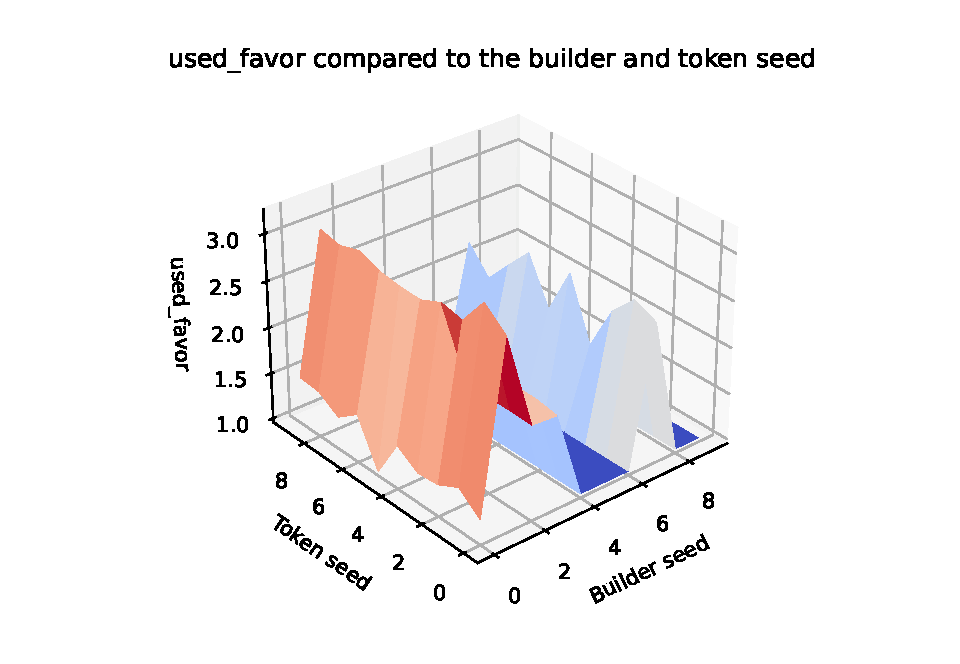
\includegraphics[width=\textwidth]{img/favor.pdf}
    \end{subfigure}
    \begin{subfigure}[b]{0.3\textwidth}
        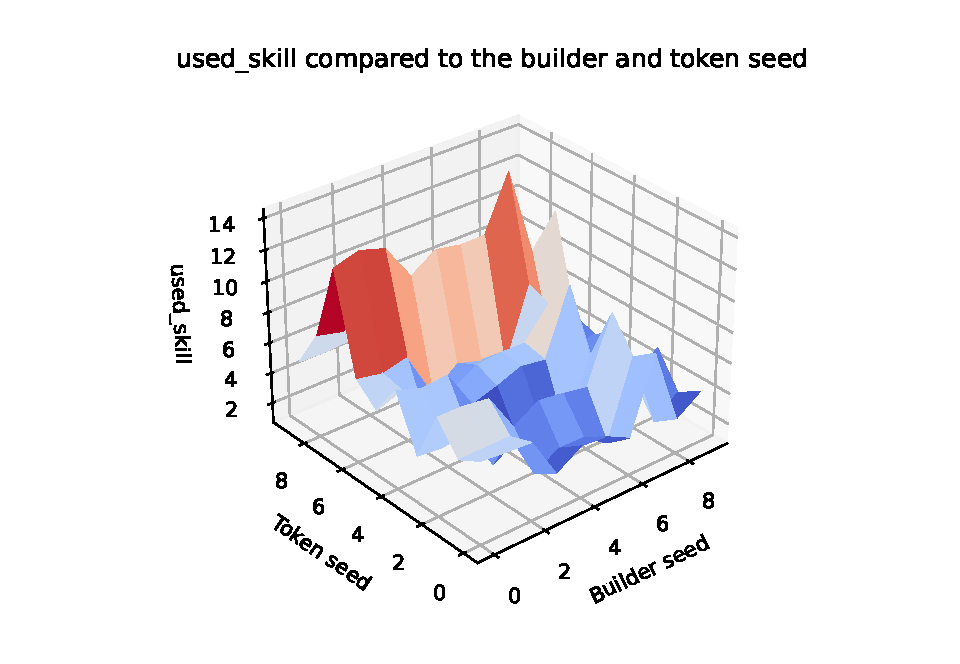
\includegraphics[width=\textwidth]{img/skills.pdf}
    \end{subfigure}
    \begin{subfigure}[b]{0.3\textwidth}
        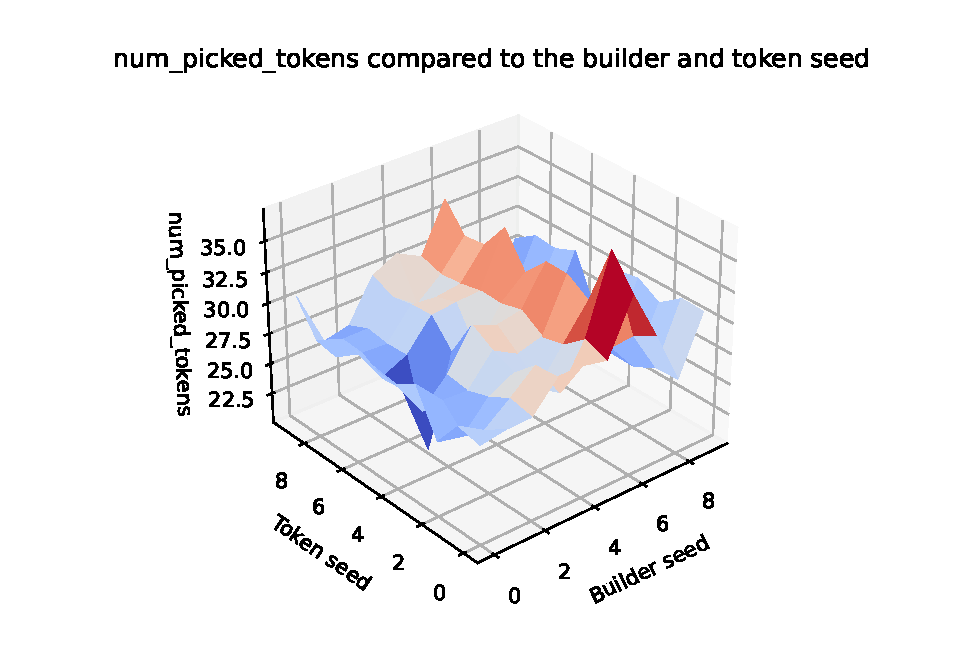
\includegraphics[width=\textwidth]{img/tokens.pdf}
    \end{subfigure} 
    \\
    \begin{subfigure}[b]{0.3\textwidth}
        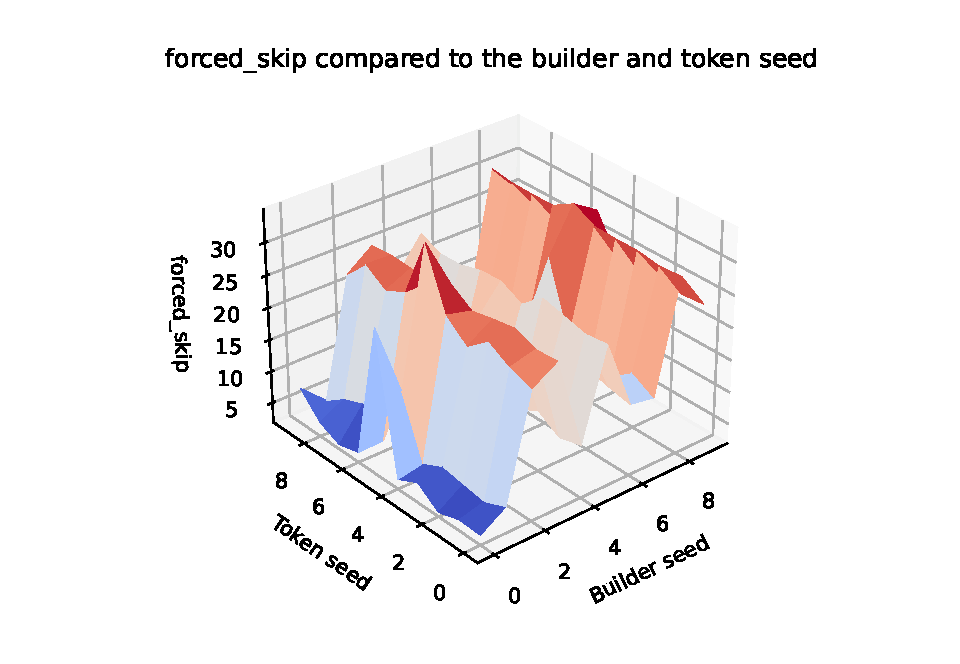
\includegraphics[width=\textwidth]{img/skip.pdf}
    \end{subfigure}
    \begin{subfigure}[b]{0.3\textwidth}
        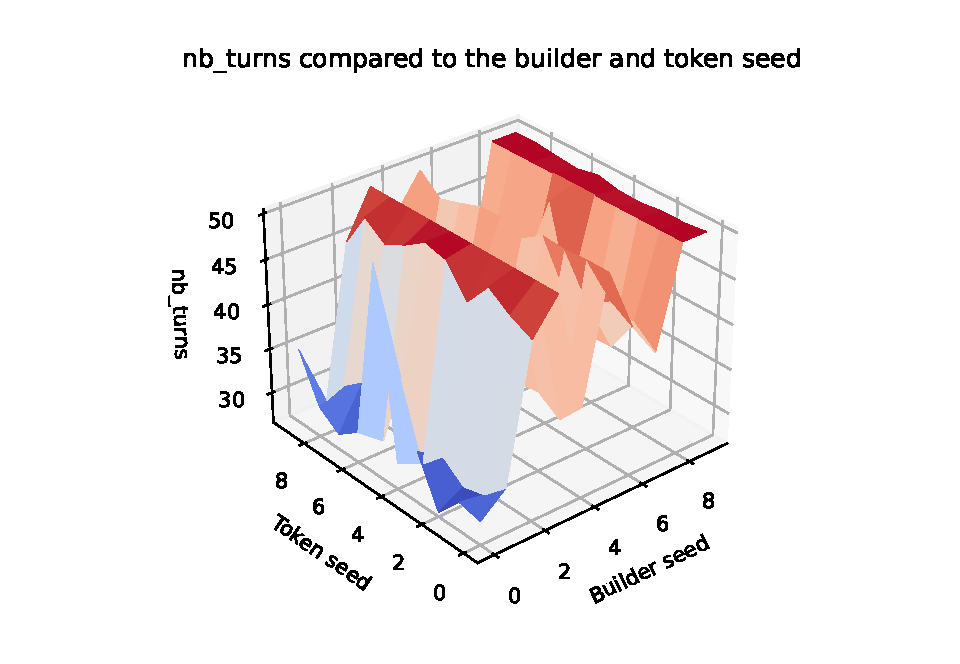
\includegraphics[width=\textwidth]{img/turns.pdf}
    \end{subfigure}
    \begin{subfigure}[b]{0.3\textwidth}
        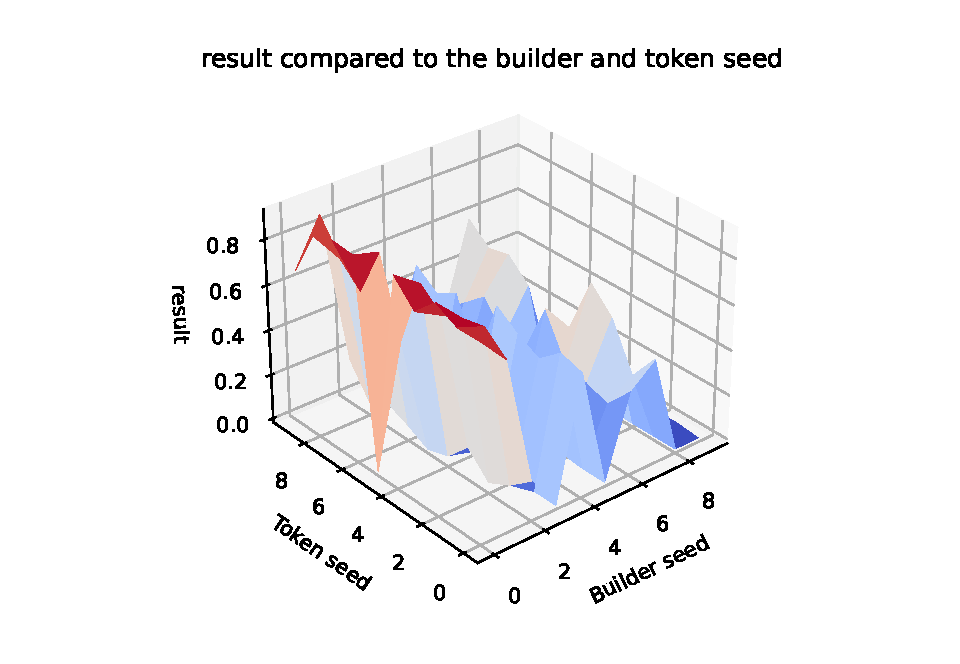
\includegraphics[width=\textwidth]{img/result.pdf}
    \end{subfigure} 
    \caption{Influence des graines sur différents paramètres de la partie}
\end{figure}
\begin{summary}
\textbf{Précision} : la graine 0 n'est pas générée aléatoirement mais correspond à un deck généré à la main afin d'avoir un jeu équilibré (selon nous).
\end{summary}
A partir de ces graphiques, on remarque un comportement intéressant : la graine des architectes a beaucoup plus d'influence sur la viabilité de la partie (beaucoup de tour et pas trop de tour passés) que celle des jetons. Par exemple on voit que les joueurs sont forcés à passer souvent leur tour avec la graine d'architecte n°3 car il y a seulement 2 architectes générés dans cette dernière.
\lstset{language=C}
\begin{lstlisting}[frame=single]
#include "fre.h"
void test(struct market_t market);
\end{lstlisting}





\end{document}